\section{Software architecture}

This section explains the application's internal structure. 

\subsection{Logical architecture}

The application's architecture is multilayered, it uses the widespread three-tier architecture. This is a clear explanation of the three-tier architecture:

\begin{quote}
    Three-tier architecture is a client-server software architecture pattern in which the user interface (presentation), functional process logic ("business rules"), computer data storage, and data access are developed and maintained as independent modules, most often on separate platforms. \cite{multitier}
\end{quote}

In the case of this project, the presentation layer is the most important one with the majority of the code. The app focuses a lot on productivity, so most of the GradeCalc's features are on its interface. The domain layer has the app's logic, and the data layer is composed of the database structure and thanks to Firebase it doesn't have any code.

% \vfill
% \begin{figure}[H]
%     \center
%     
\includegraphics[width=0.25\columnwidth]{media/layers.pdf}
%     \caption{Three tier layers.}
% \end{figure}
% \vfill

\clearpage\newpage
\subsubsection{Design patterns}
\label{sec:patterns}

Design patterns are typical solutions to common problems in software design. Each pattern is like a blueprint that you can customize to solve a particular design problem in your code.\cite{refactoring-guru}

In this section, I'm going to explain and justify the design patterns that the software of this project uses. Identifying the design patterns leads to better code because they are proved to work. Coding a custom solution certain cases may be forgotten thous introducing bugs is more frequent.

\subsubsection*{Singleton}

Singleton is a creational design pattern that lets you ensure that a class has only one instance, while providing a global access point to this instance.\cite{refactoring-guru-singleton}

This pattern is used in the database connection object as recommended by the Cloud Firestore documentation\cite{firestore-doc-init}. The code doesn't enforce the use of a singleton, but the constructor is only called once. This approach is considered a better practice because singletons inherently cause code to be tightly coupled. This makes faking them out under test rather difficult in many cases. But not enforcing the "singletoness" of the class mitigates its issues.

\subsubsection*{Proxy}

Proxy is a structural design pattern that lets you provide a substitute or placeholder for another object. A proxy controls access to the original object, allowing you to perform something either before or after the request gets through to the original object.\cite{refactoring-guru-proxy}

This pattern is used to interact with the database. There's a class that provides methods for uploading data. This is good for testing because the class can be mocked to not use the real database connections when testing certain code.

\subsubsection*{Null object}

Null object is a behavioral design pattern that avoids null references by providing a default object.

This pattern is used in the login system, when the user is not logged in, the user information object contains a default name and picture. This name and picture are displayed in the user popup.

\subsubsection*{Servant}

Servant or Utility class is a structural design pattern that defines a class with common functionality for a group of classes. The helper classes generally have no objects hence they have all static methods that act upon different kinds of class objects.

This pattern is used specially for mathematical functions like: \mintinline{js}{random(min, max)} or \mintinline{js}{round(number, decimalPlaces)}; and other kind of generic tasks like: \mintinline{js}{getRandomID()} or \mintinline{js}{isEmpty(object)}.

\subsubsection*{Adapter}

Adapter is a structural design pattern that allows objects with incompatible interfaces to collaborate.\cite{refactoring-guru-adapter}

This pattern is seamlessly used when displaying information from JSON format into HTML format because the browser can only display HTML. For example, it is used when the user searches for a subject the response obtained is a JSON object that is transformed into HTML to be displayed.



% \begin{titlebox}{TODO}
%   (3 capes, dibuix, explcacio i els patrons) three-tier architecture
% \end{titlebox}




% -----------------------------------------------------------------------------------
% -----------------------------------------------------------------------------------
% -----------------------------------------------------------------------------------
% -----------------------------------------------------------------------------------
\newpage
\subsection{Physical architecture}

% \begin{titlebox}{TODO}
%   Fill content (les 3 capes estan al frontend, i el firebase esta separat, tb netlify) (explicar com es conecta)
% \end{titlebox}

The physical architecture is heavily influenced by the choice of using Firebase. Doug Stevenson explains how firebase shapes your app's architecture very well in his Medium article "What is Firebase? The complete story, abridged."\cite{firebase-article}, this is an extract of his article:

\begin{quote}
    \onehalfspacing
    Firebase is a toolset to “build, improve, and grow your app”, and the tools it gives you cover a large portion of the services that developers would normally have to build themselves, but don’t really want to build, because they’d rather be focusing on the app experience itself. This includes things like analytics, authentication, databases, configuration, file storage, push messaging, and the list goes on. The services are hosted in the cloud, and scale with little to no effort on the part of the developer.
\end{quote}
\begin{quote}
    \onehalfspacing
    This is different than traditional app development, which typically involves writing both frontend and backend software. The frontend code just invokes API endpoints exposed by the backend, and the backend code actually does the work. However, with Firebase products, the traditional backend is bypassed, putting the work into the client.
\end{quote}

\vfill
\begin{figure}[H]
    \center
    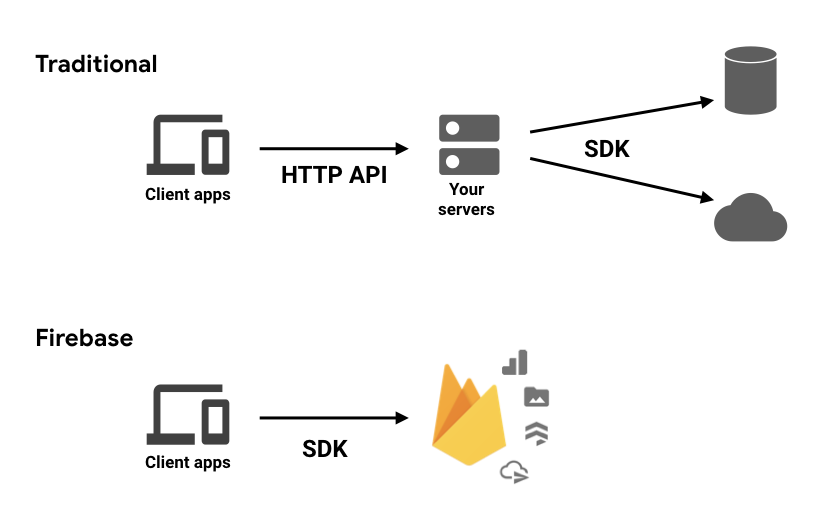
\includegraphics[width=0.95\columnwidth]{media/diagrams/firebase-diagram.png}
    \caption{Traditional vs Firebase architecture. \cite{firebase-article}}
    \label{fig:firebase-diagram}
\end{figure}
\vfill



\clearpage\newpage\noindent
The Firebase suite offers many individual products (Fig. \ref{fig:firebase-products}). The ones that this project uses are authentication and database.

\begin{figure}[H]
    \center
    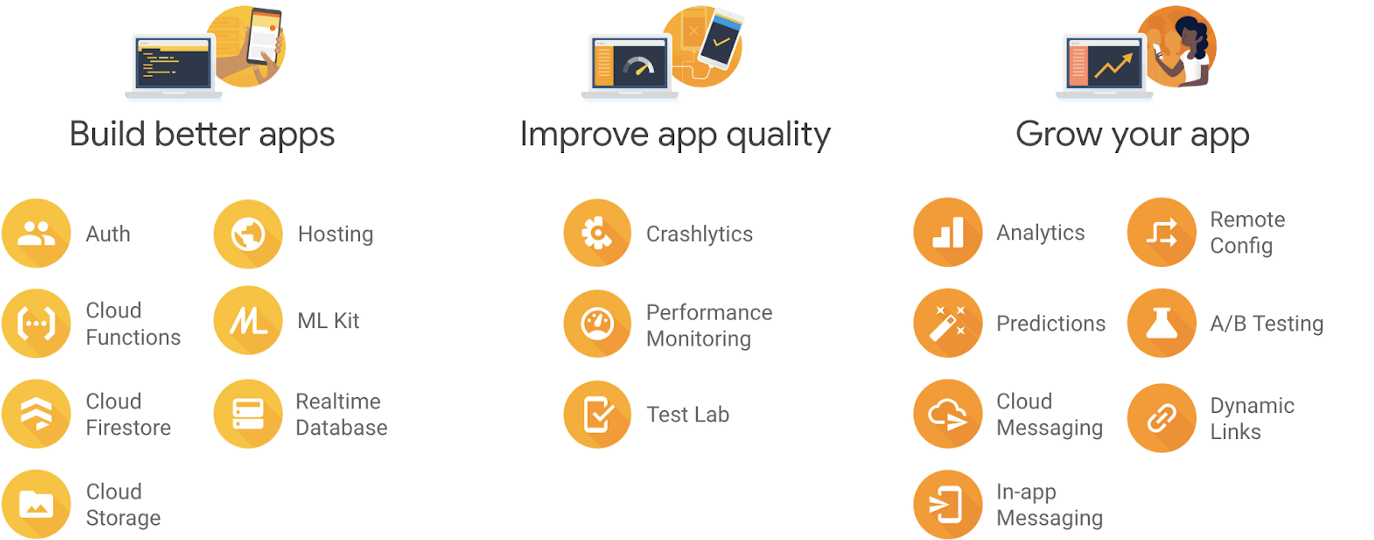
\includegraphics[width=0.95\columnwidth]{media/firebase-products-cropped.png}
    \caption{Firebase products. \cite{firebase-article}}
    \label{fig:firebase-products}
\end{figure}

% GradeCalc uses Google Firebase as the back-end, from all the features it offers, GradeCalc uses authentication and database. GradeCalc also uses Algolia, a third-party service, to perform searches. There's a cron job\footnote{A cron job is a scheduled task that runs periodically.} in Heroku that runs every day to update the searchable information in Algolia. Notice that using Firebase and Algolia allows to not have any code in the back-end, so practically speaking GradeCalc has no back-end code.

\noindent
The 3 application layers are in the front-end. There we use Gulp to generate the needed and optimized static HTML, CSS, and JS files. These optimized files are hosted in Netlify.

\vfill
\begin{figure}[H]
    \center
    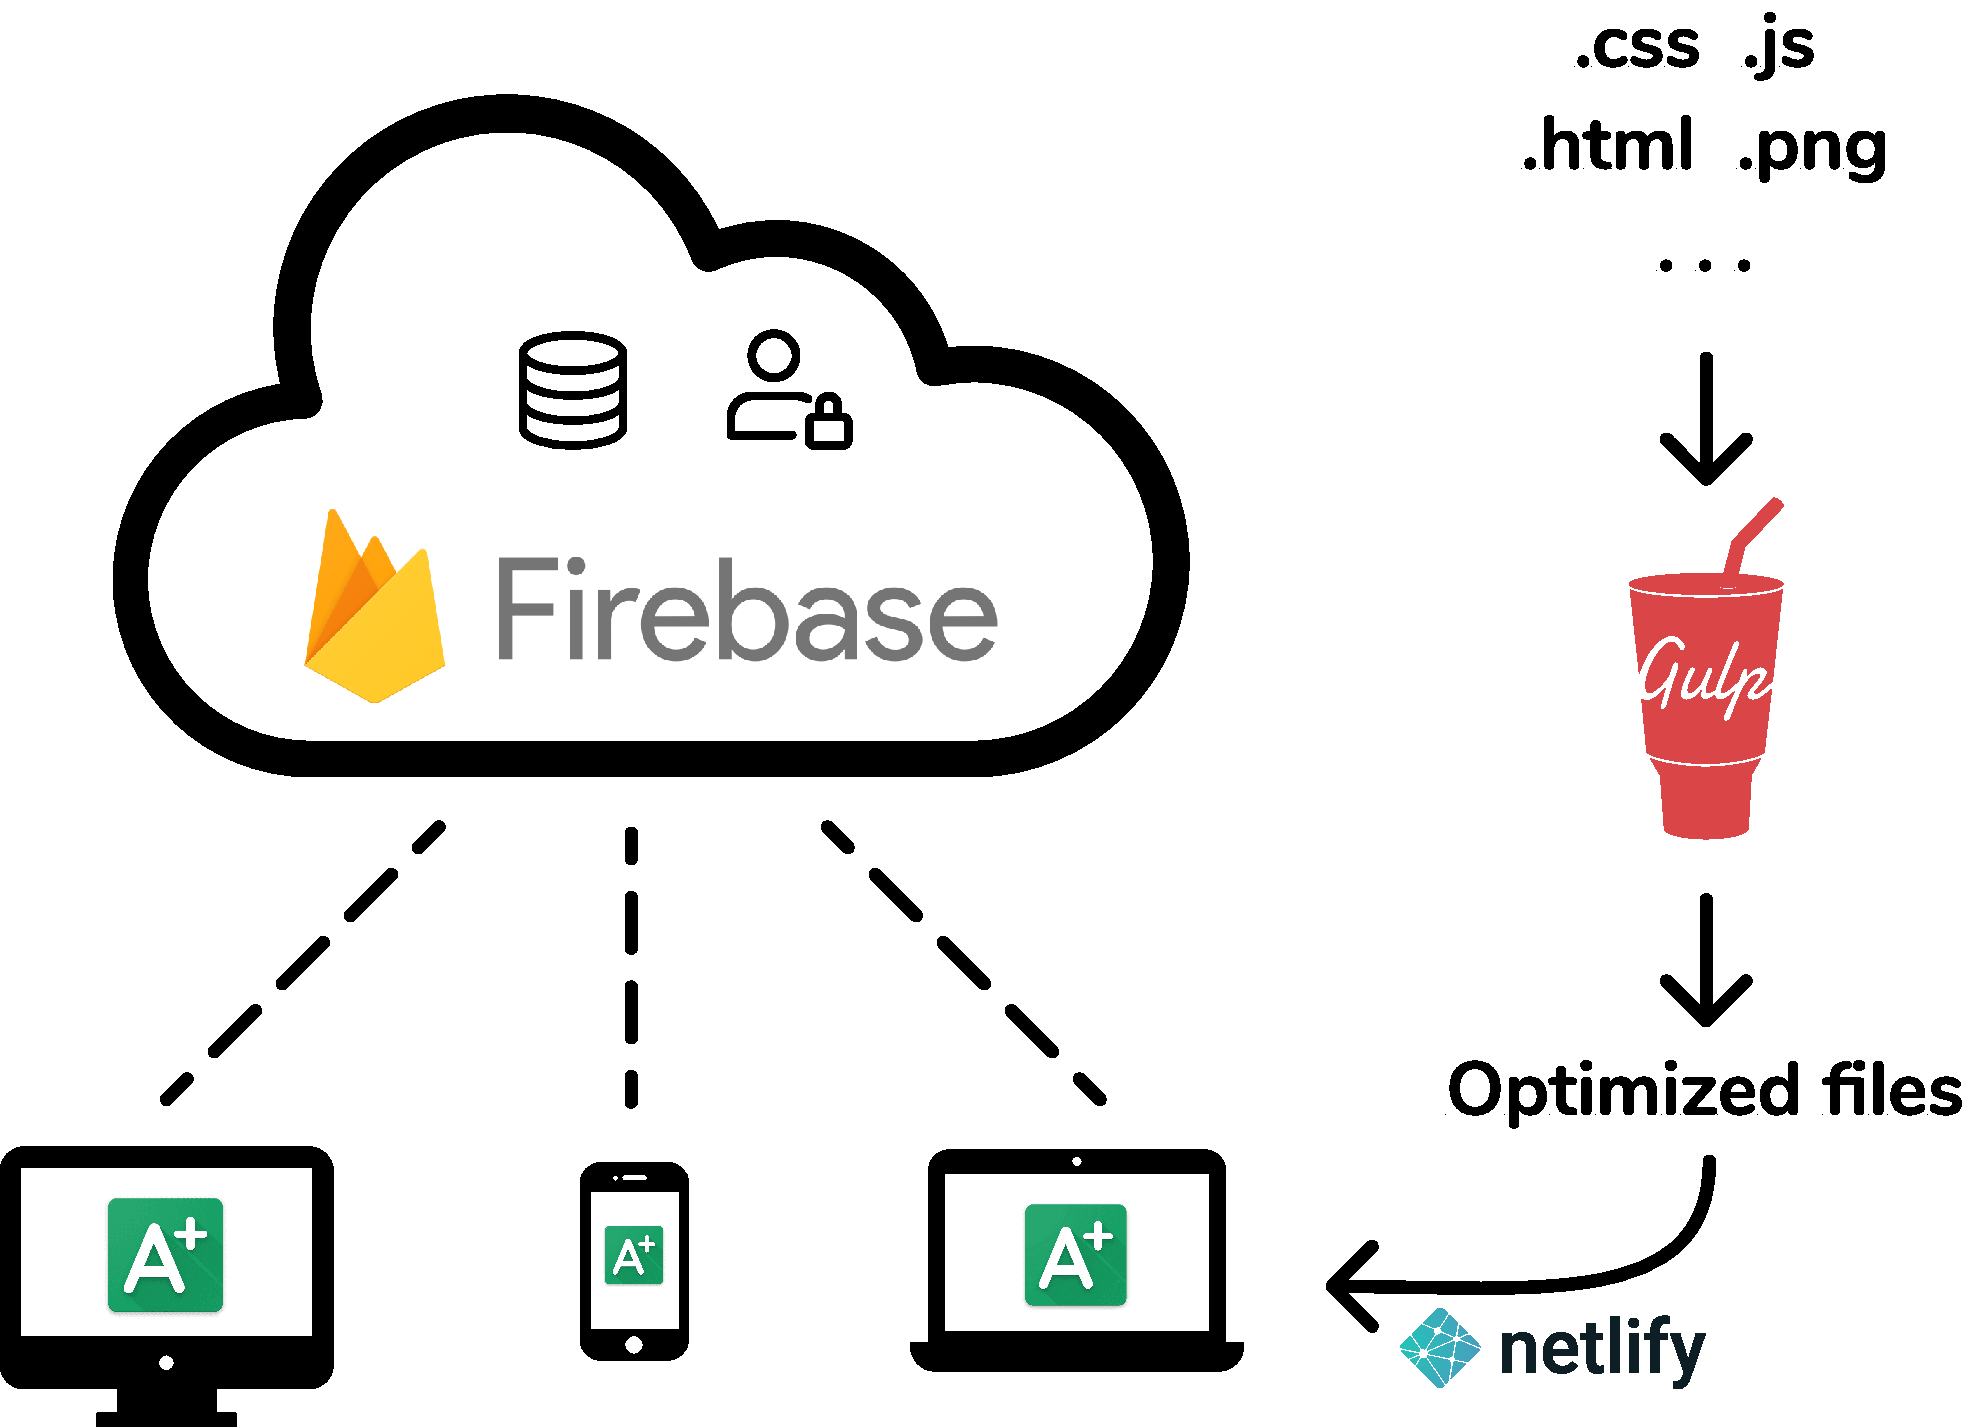
\includegraphics[width=0.85\columnwidth]{media/diagrams/architecture.pdf}
    \caption{GradeCalc architecture}
    \label{fig:architecture_diagram}
\end{figure}
\vfill





% \vfill
% \begin{figure}[H]
%     \center
%     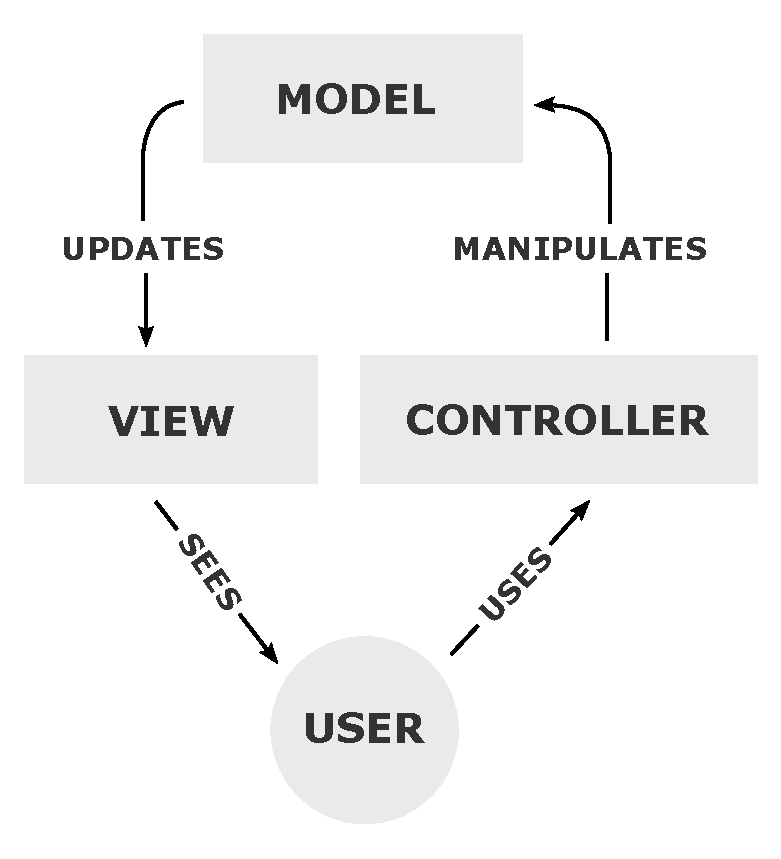
\includegraphics[width=0.5\columnwidth]{media/diagrams/MVC-Process.pdf}
%     \caption{The model, view, and controller pattern relative to the user.\cite{mvc-diagram}}
%     \label{fig:mcv-diagram}
% \end{figure}
% \vfill





\clearpage\newpage\noindent
GradeCalc is a Progressive Web App (PWA) instead of a native app. This is how Mozilla Web Docs defines PWAs \cite{pwa-mozilla}:

PWAs are web apps developed using a number of specific technologies and standard patterns to allow them to take advantage of both web and native app features. There are some key principles a web app should try to observe to be identified as a PWA. It should be:

\begin{itemize}[noitemsep]
    \item \textbf{Discoverable}, so the contents can be found through search engines.
    \item \textbf{Installable}, so it can be available on the device's home screen or app launcher.
    \item \textbf{Linkable}, so you can share it by simply sending a URL.
    \item \textbf{Network independent}, so it works offline or with a poor network connection.
    \item \textbf{Progressive}, so it's still usable on a basic level on older browsers, but fully-functional on the latest ones.
    \item \textbf{Re-engageable}, so it's able to send notifications whenever there's new content available.
    \item \textbf{Responsive}, so it's usable on any device with a screen and a browser—mobile phones, tablets, laptops, TVs, refrigerators, etc.
    \item \textbf{Safe}, so the connections between the user, the app, and your server are secured against any third parties trying to get access to sensitive data.
\end{itemize}

\noindent
Offering these features and making use of all the advantages offered by web applications can create a compelling, highly flexible offering for your users and customers.

% \subsubsection*{What is a Single-page application?}
% A single-page application (SPA) is a web application or website that interacts with the web browser by dynamically rewriting the current web page with new data from the webserver, instead of the default method of the browser loading entire new pages. The goal is faster transitions that make the website feel more like a native app.

% In a SPA, all necessary HTML, JavaScript, and CSS code is either retrieved by the browser with a single page load, or the appropriate resources are dynamically loaded and added to the page as necessary, usually in response to user actions. The page does not reload at any point in the process, nor does it transfer control to another page, although the location hash or the HTML5 History API can be used to provide the perception and navigability of separate logical pages in the application. \cite{spa}

% \subsubsection*{What is a Progressive web app?}
% Progressive Web Apps are web applications that have been designed so they are capable, reliable, and installable. These three pillars transform them into an experience that feels like a native application. \cite{pwa-pillars}
% Where:
% \begin{itemize}[noitemsep]
%     \item \textbf{Capable} means that the PWA feels as powerful/capable as a native app.
%     \item \textbf{Reliable} means that the PWA feels fast and dependable regardless of the network.
%     \item \textbf{Installable} means that the PWA runs in a standalone window instead of a browser tab
% \end{itemize}

% \subsubsection*{Why PWA instead of a native app?}

GradeCalc is PWA mainly \textbf{because it saves up a lot of development time} at the expense of some, really specific, capabilities. A PWA can run in any of the most popular operating systems (Android, iOS, Windows, macOS, and Linux), contrary to a native app that only runs in its respective OS. So, the same code will work everywhere.

% None of the app requirements (\ref{chap:requirements}) are exclusive to native apps, and some are easily achieved with a PWA.

% The main downside is that iOS users won't fully enjoy the web app\cite{pwa-ios} because Safari iOS doesn't implement some of the APIs that PWAs use, like Push Notifications. As Chris Love explains \cite{pwa-ios}:
% \begin{displayquote}
% Sure there are limitations to for Progressive Web Apps on iOS, but they are not deal breakers. Many of the most requested features have at least some form of fallback solution. It may not provide a comparable user experience the native web platform API or service offers.
% \end{displayquote}

